\documentclass{VUMIFPSkursinis}
\usepackage{algorithmicx}
\usepackage{algorithm}
\usepackage{algpseudocode}
\usepackage{amsfonts}
\usepackage{amsmath}
\usepackage{bm}
\usepackage{caption}
\usepackage{color}
\usepackage{float}
\usepackage{graphicx}
\usepackage{listings}
\usepackage{subfig}
\usepackage{wrapfig}
\usepackage{sectsty}
\usepackage{enumerate}
\usepackage{longtable}
\usepackage[export]{adjustbox}
\usepackage{rotating}
\usepackage{hhline}
\usepackage{multirow}
\usepackage{tabularx}
\usepackage{array}
\usepackage{booktabs,calc}
\usepackage{tabularx,colortbl}
\usepackage[table]{xcolor}  
\usepackage{longtable}  

\usepackage{enumitem}
%PAKEISTA, tarpai tarp sąrašo elementų
\setitemize{noitemsep,topsep=0pt,parsep=0pt,partopsep=0pt}
\setenumerate{noitemsep,topsep=0pt,parsep=0pt,partopsep=0pt}
\allsectionsfont{\centering}
% Titulinio aprašas
\university{Vilniaus universitetas}
\faculty{Matematikos ir informatikos fakultetas}
\department{Programų sistemų katedra}
\papertype{Programų sistemų inžinerijos I laboratorinis darbas}
\title{Internetinis aukcionas}
\titleineng{Digital Auction}
\status{2 kurso 4 grupės studentai}
\author{Andrejus Voitovas}
\secondauthor{Eglė Puodžiūnaitė}
\thirdauthor{Kasparas Kralikas}
\fourthauthor{Ieva Vizgirdaitė} % Pridėti antrą autorių
\supervisor{asist. dr. Vytautas Valaitis}
\date{Vilnius – \the\year}

% Nustatymai
% \setmainfont{Palemonas}   % Pakeisti teksto šriftą į Palemonas (turi būti įdiegtas sistemoje)
\bibliography{bibliografija}

\begin{document}
	% PAKEISTA
	\maketitle
	\cleardoublepage\pagenumbering{arabic}
	\setcounter{page}{2}
	\sectionnonum{ANOTACIJA}
	Šiame dokumente sistema analizuojama taikant ICONIX metodą. Pateikiami funkciniai ir nefunkciniai reikalavimai, apibrėžiamas struktūrinis dalykinės srities modelis. Taip pat aprašomos sistemoje atliekamos užduotys, analizuojami pagrindiniai ir alternatyvūs užduočių scenarijai. Rašant šį dokumentą buvo naudojamasi:
	\\1. dr. Vytauto Valaičio internetiniu puslapiu (https://klevas.mif.vu.lt/~valaitis/)
	\\2. doc., dr. Karolio Petrausko internetiniu puslapiu (http://klevas.mif.vu.lt/~karolis/)
	\\3. Latex programa
	\\4. lab. asst. Jono Brusoko parengtais kursinio darbo šablonais (https://gitlab.com/JohnLogic/SE-course-work-template)
	\newpage
	%TURINYS
	\tableofcontents
	
	\sectionnonum{ĮVADAS}
	Internetinis aukcionas kuriamas siekiant išplėsti dalyvavimą aukcionuose nuotoliniu
	būdu. Tinklalapis suteikia galimybę klientams paprastai ir patogiai dalyvauti aukcionuose bet kuriuo paros metu. Dokumente pateikiamas pagrindinis programos funkcionalumas ir tam tikri ribojimai jos kūrimui. Pasitelkiant ICONIX metodą sudaromi užduočių scenarijai, apibrėžiamos pagrindinės kuriamos sistemos esybės, sudaromas struktūrinis dalykinės srities modelis. Šis dokumentas padeda toliau projektuoti ir nuspręsti, kaip sistema turėtų būti įgyvendinta.
	\\\textbf{Dalykinė sritis}
	\\Internetinis aukcionas.
	\\\textbf{Probleminė sritis} 
	\\Internetinis aukcionas suteiktų galimybę greitai ir paprastai dalyvauti aukcionuose.
	\\\textbf{Darbo pagrindas}
	\\Dokumentas parengtas kaip Programų sistemų inžinerijos II dalies I laboratorinis darbas.
	\\\textbf{Darbo užduotys}
	\\1. Suformuluoti funkcinius reikalavimus.
	\\2. Suformuluoti nefunkcinius reikalavimus.
	\\3. Apibrėžti struktūrinį dalykinės srities modelį.
	\\4. Aprašyti sistemoje atliekamas užduotis.
	\newpage
	\section{FUNKCINIAI REIKALAVIMAI}
	Šiame skyriuje pateikiami funkciniai reikalavimai – nagrinėjami scenarijai, ką sistema turi daryti, kaip elgtis vienu ar kitu atveju.
	
	\subsection{Internetinės svetainės langai}
	\begin{table}[H]
		\caption{Funkciniai reikalavimai. Internetinės svetainės langai.}
		\begin{tabular}{|p{1cm}|p{1cm}|p{11,5cm}|p{3,5cm}|}
			\hline 
			\rowcolor{gray!50}
			\multicolumn{2}{|c|}{{\bfseries Kodas}}&
			\multicolumn{1}{c|}{{\bfseries Reikalavimas}}&
			\multicolumn{1}{c|}{{\bfseries Svarba}}\\
			\hline
			\rowcolor{lightgray}
			\multicolumn{4}{|c|}{Internetinės svetainės langai}\\		
			
			\hline
			\multicolumn{2}{|c|}{FR 1.1}&
			{Svetainės langai „Registracija“, „Prisijungimas“, „Pagrindinis puslapis“, „Taisyklės“ turi būti matomi visiems naudotojams.
			}&		
			\multicolumn{1}{c|}{Būtina}\\
			\hline
			\multicolumn{1}{|c}{}&
			\multicolumn{1}{c|}{FR 1.2}&
			{Svetainės langai „Mano profilis“, „Prekės įkėlimas“, „Prekės aukcionas“ turi būti matomi visiems prisijungusiems naudotojams.
			}&		
			\multicolumn{1}{c|}{Būtina}\\
			\hline
			\multicolumn{1}{|c}{}&
			\multicolumn{1}{c|}{FR 1.3}&
			{Svetainės langai „Visi aukcionai“, „Naudotojai“  turi būti matomas sistemos adminstratoriams.
			}&
			\multicolumn{1}{c|}{Būtina}\\	
			\hline		
		\end{tabular}		
	\end{table}
	
	\subsection{Registracija}
	\begin{table}[H]
		\caption{Funkciniai reikalavimai. Registracija.}
		\begin{tabular}{|p{1cm}|p{1cm}|p{11,5cm}|p{3,5cm}|}
			\hline 
			\rowcolor{gray!50}
			\multicolumn{2}{|c|}{{\bfseries Kodas}}&
			\multicolumn{1}{c|}{{\bfseries Reikalavimas}}&
			\multicolumn{1}{c|}{{\bfseries Svarba}}\\
			\hline
			\rowcolor{lightgray}
			\multicolumn{4}{|c|}{Registracija}\\		
			
			\hline
			\multicolumn{2}{|c|}{FR 2.1}&
			{Naudotojui suvedus visą reikiamą informaciją ir nuspaudus mygtuką registruotis, jis turi būti priregistruojamas internetinėje sveitainėje.
			}&		
			\multicolumn{1}{c|}{Būtina}\\
			\hline
			\multicolumn{1}{|c}{}&
			\multicolumn{1}{c|}{FR 2.2}&
			{Naudotojui nesuvedus informacijos į visus privalomus laukus jis neturi būti priregistruojamas sistemoje bei registracijos puslapyje turi būti išmetamas klaidos pranešimas, pranešantis, jog reikia užpildyti visus privalomus laukus.
			}&		
			\multicolumn{1}{c|}{Būtina}\\
			\hline	
			\multicolumn{1}{|c}{}&
			\multicolumn{1}{c|}{FR 2.3}&
			{Registruojantis naudotojas turi įvesti internetinėje svetainėje dar nepriregistruotą el. pašto adresą.
			}&
			\multicolumn{1}{c|}{Būtina}\\									
			\hline
		\end{tabular}		
	\end{table}
	
	\subsection{Prisijungimas}
	\begin{table}[H]
		\caption{Funkciniai reikalavimai. Prisijungimas.}
		\begin{tabular}{|p{1cm}|p{1cm}|p{11,5cm}|p{3,5cm}|}
			\hline 
			\rowcolor{gray!50}
			\multicolumn{2}{|c|}{{\bfseries Kodas}}&
			\multicolumn{1}{c|}{{\bfseries Reikalavimas}}&
			\multicolumn{1}{c|}{{\bfseries Svarba}}\\
			\hline
			\rowcolor{lightgray}
			\multicolumn{4}{|c|}{Prisijungimas}\\		
			
			\hline
			\multicolumn{2}{|c|}{FR 3.1}&
			{Naudotojui suvedus tinkamus prisijungimo duomenis jis turi būti prijungiamas prie sistemos.
			}&		
			\multicolumn{1}{c|}{Būtina}\\
			\hline
			\multicolumn{1}{|c}{}&
			\multicolumn{1}{c|}{FR 3.2}&
			{Naudotojui netinkamai įvedus prisijungimo duomenis jis neturi būti prijungiamas prie sistemos bei turi būti išmetamas klaidos pranešimas.
			}&		
			\multicolumn{1}{c|}{Būtina}\\
			\hline	
			\multicolumn{1}{|c}{}&
			\multicolumn{1}{c|}{FR 3.3}&
			{Naudotojo bandymų prisijungti prie sistemos skaičius neturi būti ribojamas.
			}&
			\multicolumn{1}{c|}{Būtina}\\									
			\hline
		\end{tabular}		
	\end{table}
	
	\subsection{Atsijungimas}
	
	\begin{table}[H]
		\caption{Funkciniai reikalavimai. Atsijungimas.}
		\begin{tabular}{|p{1cm}|p{1cm}|p{11,5cm}|p{3,5cm}|}
			\hline 
			\rowcolor{gray!50}
			\multicolumn{2}{|c|}{{\bfseries Kodas}}&
			\multicolumn{1}{c|}{{\bfseries Reikalavimas}}&
			\multicolumn{1}{c|}{{\bfseries Svarba}}\\
			\hline
			\rowcolor{lightgray}
			\multicolumn{4}{|c|}{Atsijungimas}\\		
			
			\hline
			\multicolumn{2}{|c|}{FR 4.1}&
			{Naudotojas paspaudęs mygtuką atsijungti turi būti atjungiamas nuo sistemos.
			}&		
			\multicolumn{1}{c|}{Būtina}\\
			\hline
		\end{tabular}		
	\end{table}
	
	\subsection{Paskyros valdymas}
	
	\begin{table}[H]
		\caption{Funkciniai reikalavimai. Paskyros valdymas.}
		\begin{tabular}{|p{1cm}|p{1cm}|p{11,5cm}|p{3,5cm}|}
			\hline 
			\rowcolor{gray!50}
			\multicolumn{2}{|c|}{{\bfseries Kodas}}&
			\multicolumn{1}{c|}{{\bfseries Reikalavimas}}&
			\multicolumn{1}{c|}{{\bfseries Svarba}}\\
			\hline
			\rowcolor{lightgray}
			\multicolumn{4}{|c|}{Paskyros valdymas}\\				
			\hline
			\multicolumn{2}{|c|}{FR 5.1}&
			{Naudotojui paspaudus mygtuką „Mano profilis“ turi būti matoma visa žinoma informacija apie naudotoją.
			}&		
			\multicolumn{1}{c|}{Būtina}\\
			\hline
			\multicolumn{1}{|c}{}&
			\multicolumn{1}{c|}{FR 5.2}&
			{Naudotojui paspaudus mygtuką „Pakeisti slaptažodį“, įvedus tinkamą seną ir naują slaptažodžius bei paspaudus mygtuką „Patvirtinti“ slaptažodis turi būti pakeičiamas į naują.
			}&		
			\multicolumn{1}{c|}{Būtina}\\
			\hline
			\multicolumn{1}{|c}{}&
			\multicolumn{1}{c|}{FR 5.3}&
			{Naudotojui paspaudus mygtuką „Pakeisti slaptažodį“ ir įvedus netinkamą seną slaptažodį turi būti išvedamas klaidos pranešimas.
			}&
			\multicolumn{1}{c|}{Būtina}\\	
			\hline		
		\end{tabular}		
	\end{table}
	
	\subsection{Taisyklės}
	\begin{table}[H]
		\caption{Funkciniai reikalavimai. Taisyklės}
		\begin{tabular}{|p{1cm}|p{1cm}|p{11,5cm}|p{3,5cm}|}
			\hline 
			\rowcolor{gray!50}
			\multicolumn{2}{|c|}{{\bfseries Kodas}}&
			\multicolumn{1}{c|}{{\bfseries Reikalavimas}}&
			\multicolumn{1}{c|}{{\bfseries Svarba}}\\
			\hline
			\rowcolor{lightgray}
			\multicolumn{4}{|c|}{Taisyklės}\\		
			
			\hline
			\multicolumn{2}{|c|}{FR 6.1}&
			{Taisyklės turi būti matomos puslapyje „Taisyklės“.
			}&		
			\multicolumn{1}{c|}{Būtina}\\
			\hline
			\multicolumn{1}{|c}{}&
			\multicolumn{1}{c|}{FR 6.2}&
			{Visas taisyklių sąrašas turi būti pateikiamas viename puslapyje.
			}&		
			\multicolumn{1}{c|}{Būtina}\\
			\hline	
			\multicolumn{1}{|c}{}&
			\multicolumn{1}{c|}{FR 6.3}&
			{Taisyklės turi būti matomos visiems sistemos naudotojams.
			}&
			\multicolumn{1}{c|}{Būtina}\\									
			\hline
		\end{tabular}		
	\end{table}
	
	\subsection{Pagrindinis puslapis}
	\begin{table}[H]
		\caption{Funkciniai reikalavimai. Pagrindinis puslapis}
		\begin{tabular}{|p{1cm}|p{1cm}|p{11,5cm}|p{3,5cm}|}
			\hline 
			\rowcolor{gray!50}
			\multicolumn{2}{|c|}{{\bfseries Kodas}}&
			\multicolumn{1}{c|}{{\bfseries Reikalavimas}}&
			\multicolumn{1}{c|}{{\bfseries Svarba}}\\
			\hline
			\rowcolor{lightgray}
			\multicolumn{4}{|c|}{Pagrindinis puslapis}\\		
			
			\hline
			\multicolumn{2}{|c|}{FR 7.1}&
			{Aktyvūs aukcionai turi būti matomi puslapyje „Pagrindinis puslapis“.
			}&		
			\multicolumn{1}{c|}{Būtina}\\
			\hline
			\multicolumn{1}{|c}{}&
			\multicolumn{1}{c|}{FR 7.2}&
			{Visas aktyvių aukcionų sąrašas turi būti pateikiamas viename puslapyje.
			}&		
			\multicolumn{1}{c|}{Būtina}\\
			\hline	
			\multicolumn{1}{|c}{}&
			\multicolumn{1}{c|}{FR 7.3}&
			{Pagrindinis puslapis turi būti matomas visiems sistemos naudotojams.
			}&
			\multicolumn{1}{c|}{Būtina}\\									
			\hline
			\multicolumn{1}{|c}{}&
			\multicolumn{1}{c|}{FR 7.4}&
			{Prisijungusiam naudotojui paspaudus ant aktyvaus aukciono mygtuko „Daugiau informacijos“ turi būti atidaromas puslapis „Prekės aukcionas“.
			}&
			\multicolumn{1}{c|}{Būtina}\\									
			\hline
		\end{tabular}		
	\end{table}
	
	\subsection{Prekės įkėlimas}
	\begin{table}[H]
		\caption{Funkciniai reikalavimai. Prekės įkėlimas}
		\begin{tabular}{|p{1cm}|p{1cm}|p{11,5cm}|p{3,5cm}|}
			\hline 
			\rowcolor{gray!50}
			\multicolumn{2}{|c|}{{\bfseries Kodas}}&
			\multicolumn{1}{c|}{{\bfseries Reikalavimas}}&
			\multicolumn{1}{c|}{{\bfseries Svarba}}\\
			\hline
			\rowcolor{lightgray}
			\multicolumn{4}{|c|}{Prekės įkėlimas}\\		
			
			\hline
			\multicolumn{2}{|c|}{FR 8.1}&
			{Puslapis „Prekės įkėlimas“ turi būti matomas visiems prijungusiems naudotojams.
			}&		
			\multicolumn{1}{c|}{Būtina}\\
			\hline
			\multicolumn{1}{|c}{}&
			\multicolumn{1}{c|}{FR 8.2}&
			{Naudotojui suvedus visą reikiamą informaciją apie aukciono prekę bei paspaudus mygtuką „Patvirtinti“ turi būti sukuriamas aukcionas.
			}&		
			\multicolumn{1}{c|}{Būtina}\\
			\hline	
			\multicolumn{1}{|c}{}&
			\multicolumn{1}{c|}{FR 8.3}&
			{Naudotojui nesuvedus informacijos į visus privalomus laukus aukcionas neturi būti sukuriamas bei prekės įkėlimo puslapyje turi būti išmetamas klaidos pranešimas, pranešantis, jog reikia užpildyti visus privalomus laukus.
			}&
			\multicolumn{1}{c|}{Būtina}\\									
			\hline
		\end{tabular}		
	\end{table}
	
	\subsection{Prekės aukcionas}
	\begin{table}[H]
		\caption{Funkciniai reikalavimai. Prekės aukcionas}
		\begin{tabular}{|p{1cm}|p{1cm}|p{11,5cm}|p{3,5cm}|}
			\hline 
			\rowcolor{gray!50}
			\multicolumn{2}{|c|}{{\bfseries Kodas}}&
			\multicolumn{1}{c|}{{\bfseries Reikalavimas}}&
			\multicolumn{1}{c|}{{\bfseries Svarba}}\\
			\hline
			\rowcolor{lightgray}
			\multicolumn{4}{|c|}{Prekės aukcionas}\\				
			\hline
			\multicolumn{2}{|c|}{FR 9.1}&
			{Puslapis „Prekės aukcionas“ turi būti matomas visiems prijungusiems naudotojams.
			}&		
			\multicolumn{1}{c|}{Būtina}\\
			\hline
			\multicolumn{1}{|c}{}&
			\multicolumn{1}{c|}{FR 9.2}&
			{Puslapyje „Prekės aukcionas“ aukcionas yra aktyvus tokį laikotarpį, kokį nurodė naudotojas sukūręs aukcioną.
			}&		
			\multicolumn{1}{c|}{Būtina}\\
			\hline	
			\multicolumn{1}{|c}{}&
			\multicolumn{1}{c|}{FR 9.3}&
			{Jei aukciono statusas yra „Aktyvus“ naudotojai gali siūlyti savo kainas jas įvedus į kainos laukelį ir paspaudus mygtuką „Patvirtinti“.
			}&
			\multicolumn{1}{c|}{Būtina}\\									
			\hline
			\multicolumn{1}{|c}{}&
			\multicolumn{1}{c|}{FR 9.4}&
			{Naudotojo siūloma kaina negali būti mažesnė už jau pasiūlytą kainą. Jei naudotojas bando pasiūlyti mažesnę kainą, turi būti išmetamas klaidos pranešimas, jog kaina yra per maža.
			}&
			\multicolumn{1}{c|}{Būtina}\\									
			\hline
			\multicolumn{1}{|c}{}&
			\multicolumn{1}{c|}{FR 9.5}&
			{Praėjus naudotojo nurodytam aukciono laikotarpiui jo statusas turi automatiškai pasikeisti į „Pasibaigęs“, puslapyje „Prekės aukcionas“ turi būti parašytas aukciono laimėtojas, o kainos siūlymo laukelis nebeturi būti matomas.
			}&
			\multicolumn{1}{c|}{Būtina}\\									
			\hline
		\end{tabular}		
	\end{table}
	
	\subsection{Visi aukcionai}
	\begin{table}[H]
		\caption{Funkciniai reikalavimai. Visi aukcionai}
		\begin{tabular}{|p{1cm}|p{1cm}|p{11,5cm}|p{3,5cm}|}
			\hline 
			\rowcolor{gray!50}
			\multicolumn{2}{|c|}{{\bfseries Kodas}}&
			\multicolumn{1}{c|}{{\bfseries Reikalavimas}}&
			\multicolumn{1}{c|}{{\bfseries Svarba}}\\
			\hline
			\rowcolor{lightgray}
			\multicolumn{4}{|c|}{Visi aukcionai}\\				
			\hline
			\multicolumn{2}{|c|}{FR 10.1}&
			{Puslapis „Visi aukcionai“ turi būti matomas tik sistemos administratoriams.
			}&		
			\multicolumn{1}{c|}{Būtina}\\
			\hline
			\multicolumn{1}{|c}{}&
			\multicolumn{1}{c|}{FR 10.2}&
			{Puslapyje „Visi aukcionai“ turi būti matomas visų aktyvių ir pasibaigusių aukcionų sąrašas.
			}&		
			\multicolumn{1}{c|}{Būtina}\\
			\hline	
			\multicolumn{1}{|c}{}&
			\multicolumn{1}{c|}{FR 10.3}&
			{Visas aukcionų sąrašas turi būti pateikiamas viename puslapyje.
			}&
			\multicolumn{1}{c|}{Būtina}\\									
			\hline
			\multicolumn{1}{|c}{}&
			\multicolumn{1}{c|}{FR 10.4}&
			{Puslapyje administratorius turi turėti galimybę ištrinti aukcioną.
			}&
			\multicolumn{1}{c|}{Būtina}\\									
			\hline
		\end{tabular}		
	\end{table}
	
	\subsection{Naudotojai}
	\begin{table}[H]
		\caption{Funkciniai reikalavimai. Naudotojai}
		\begin{tabular}{|p{1cm}|p{1cm}|p{11,5cm}|p{3,5cm}|}
			\hline 
			\rowcolor{gray!50}
			\multicolumn{2}{|c|}{{\bfseries Kodas}}&
			\multicolumn{1}{c|}{{\bfseries Reikalavimas}}&
			\multicolumn{1}{c|}{{\bfseries Svarba}}\\
			\hline
			\rowcolor{lightgray}
			\multicolumn{4}{|c|}{Naudotojai}\\				
			\hline
			\multicolumn{2}{|c|}{FR 11.1}&
			{Puslapis „Naudotojai“ turi būti matomas tik sistemos administratoriams.
			}&		
			\multicolumn{1}{c|}{Būtina}\\
			\hline
			\multicolumn{1}{|c}{}&
			\multicolumn{1}{c|}{FR 11.2}&
			{Puslapyje „Naudotojai“ turi būti matomas visų naudotojų sąrašas.
			}&		
			\multicolumn{1}{c|}{Būtina}\\
			\hline	
			\multicolumn{1}{|c}{}&
			\multicolumn{1}{c|}{FR 11.3}&
			{Visas naudotojų sąrašas turi būti pateikiamas viename puslapyje.
			}&
			\multicolumn{1}{c|}{Būtina}\\									
			\hline
			\multicolumn{1}{|c}{}&
			\multicolumn{1}{c|}{FR 11.4}&
			{Puslapyje administratorius turi turėti galimybę užblokuoti naudotoją.
			}&
			\multicolumn{1}{c|}{Būtina}\\									
			\hline
		\end{tabular}		
	\end{table}
	
	\subsection{Sąskaita}
	\begin{table}[H]
		\caption{Funkciniai reikalavimai. Sąskaita}
		\begin{tabular}{|p{1cm}|p{1cm}|p{11,5cm}|p{3,5cm}|}
			\hline 
			\rowcolor{gray!50}
			\multicolumn{2}{|c|}{{\bfseries Kodas}}&
			\multicolumn{1}{c|}{{\bfseries Reikalavimas}}&
			\multicolumn{1}{c|}{{\bfseries Svarba}}\\
			\hline
			\rowcolor{lightgray}
			\multicolumn{4}{|c|}{Sąskaita}\\				
			\hline
			\multicolumn{2}{|c|}{FR 11.1}&
			{Kiekvienas prisiregistravęs sistemos naudotojas turi turėti savo sąskaitą.
			}&		
			\multicolumn{1}{c|}{Būtina}\\
			\hline
			\multicolumn{1}{|c}{}&
			\multicolumn{1}{c|}{FR 11.2}&
			{Naudotojo sąskaitos likutis turi būti matomas puslapyje „Mano profilis“.
			}&		
			\multicolumn{1}{c|}{Būtina}\\
			\hline	
			\multicolumn{1}{|c}{}&
			\multicolumn{1}{c|}{FR 11.3}&
			{Kiekvienas prisiregistravęs sistemos naudotojas turi turėti galimybę papildyti savo sąskaitą.
			}&
			\multicolumn{1}{c|}{Būtina}\\									
			\hline
			\multicolumn{1}{|c}{}&
			\multicolumn{1}{c|}{FR 11.4}&
			{Naudotojas dalyvaudamas aukcione negali statyti didesnės pinigų sumos, negu turi savo sąskaitoje.
			}&
			\multicolumn{1}{c|}{Būtina}\\									
			\hline
		\end{tabular}		
	\end{table}
	\newpage
	
	\section{NEFUNKCINIAI REIKALAVIMAI}
	
	\subsection{Programinės įrangos bei techniniai reikalavimai}
	\begin{table}[H]
		\caption{Nefunkciniai reikalavimai. PĮ}
		\begin{tabular}{|p{1cm}|p{1cm}|p{11,5cm}|p{3,5cm}|}
			\hline 
			\rowcolor{gray!50}
			\multicolumn{2}{|c|}{{\bfseries Kodas}}&
			\multicolumn{1}{c|}{{\bfseries Reikalavimas}}&
			\multicolumn{1}{c|}{{\bfseries Svarba}}\\
			\hline
			\rowcolor{lightgray}
			\multicolumn{4}{|c|}{PĮ ir techniniai reikalvimai}\\				
			\hline
			\multicolumn{2}{|c|}{NFR 1.1}&
			{Naudojama MySQL duomenų bazių valdymo sistema. 
			}&		
			\multicolumn{1}{c|}{Būtina}\\
			\hline
			\multicolumn{1}{|c}{}&
			\multicolumn{1}{c|}{NFR 1.2}&
			{Duomenų bazėje saugoma informacija apie registruotus vartotojus, prekes.
			}&		
			\multicolumn{1}{c|}{Būtina}\\
			\hline	
		\end{tabular}		
	\end{table}
	
	\subsection{Programavimo kalbos reikalavimai}
	\begin{table}[H]
		\caption{Nefunkciniai reikalavimai. Programavimo kalbos reikalavimai}
		\begin{tabular}{|p{1cm}|p{1cm}|p{11,5cm}|p{3,5cm}|}
			\hline 
			\rowcolor{gray!50}
			\multicolumn{2}{|c|}{{\bfseries Kodas}}&
			\multicolumn{1}{c|}{{\bfseries Reikalavimas}}&
			\multicolumn{1}{c|}{{\bfseries Svarba}}\\
			\hline
			\rowcolor{lightgray}
			\multicolumn{4}{|c|}{Programavimo kalbos reikalvimai}\\				
			\hline
			\multicolumn{2}{|c|}{NFR 2.1}&
			{Programa kuriama Javascript programavimo kalba.}&		
			\multicolumn{1}{c|}{Būtina}\\
			\hline
		\end{tabular}		
	\end{table}
	
	\subsection{Programavimo aplinkos reikalavimai}
	\begin{table}[H]
		\caption{Nefunkciniai reikalavimai. Programavimo aplinkos reikalavimai}
		\begin{tabular}{|p{1cm}|p{1cm}|p{11,5cm}|p{3,5cm}|}
			\hline 
			\rowcolor{gray!50}
			\multicolumn{2}{|c|}{{\bfseries Kodas}}&
			\multicolumn{1}{c|}{{\bfseries Reikalavimas}}&
			\multicolumn{1}{c|}{{\bfseries Svarba}}\\
			\hline
			\rowcolor{lightgray}
			\multicolumn{4}{|c|}{Programavimo aplinkos reikalvimai}\\				
			\hline
			\multicolumn{2}{|c|}{NFR 3.1}&
			{Programa kuriama Webstorm programavimo aplinkoje.}&		
			\multicolumn{1}{c|}{Pageidautina}\\
			\hline
			\multicolumn{2}{|c|}{NFR 3.2}&
			{Kodo saugojimui ir dalinimuisi naudojama privati Github repositorija.}&		
			\multicolumn{1}{c|}{Būtina}\\
			\hline
		\end{tabular}		
	\end{table}
	
	\subsection{Vaizdavimo tikslumo reikalavimai}
	\begin{table}[H]
		\caption{Nefunkciniai reikalavimai. Vaizdavimo tikslumo reikalavimai}
		\begin{tabular}{|p{1cm}|p{1cm}|p{11,5cm}|p{3,5cm}|}
			\hline 
			\rowcolor{gray!50}
			\multicolumn{2}{|c|}{{\bfseries Kodas}}&
			\multicolumn{1}{c|}{{\bfseries Reikalavimas}}&
			\multicolumn{1}{c|}{{\bfseries Svarba}}\\
			\hline
			\rowcolor{lightgray}
			\multicolumn{4}{|c|}{Vaizdavimo tikslumo reikalvimai}\\				
			\hline
			\multicolumn{2}{|c|}{NFR 4.1}&
			{Prekės antraštė, pavadinimas - iki 20 simbolių.}&		
			\multicolumn{1}{c|}{Būtina}\\
			\hline
			\multicolumn{2}{|c|}{NFR 4.2}&
			{Prekės kaina - centų tikslumu}&		
			\multicolumn{1}{c|}{Būtina}\\
			\hline
			\multicolumn{2}{|c|}{NFR 4.3}&
			{Prekės paveikslėlis - PNG arba JPG formatu.}&		
			\multicolumn{1}{c|}{Būtina}\\
			\hline
			\multicolumn{2}{|c|}{NFR 4.4}&
			{Prekės paveikslėlio failo dydis - ne daugiau 4MB.}&		
			\multicolumn{1}{c|}{Būtina}\\
			\hline
			\multicolumn{2}{|c|}{NFR 4.5}&
			{Prekės aprašas - ne daugiau 500 simbolių.}&		
			\multicolumn{1}{c|}{Būtina}\\
			\hline
			\multicolumn{2}{|c|}{NFR 4.6}&
			{Aukciono dienos pasirinkimas - 1 diena, 3 dienos, savaitė.}&		
			\multicolumn{1}{c|}{Būtina}\\
			\hline
			\multicolumn{2}{|c|}{NFR 4.7}&
			{Laiko formatas - HH:MM:SS, kur HH - valandos, MM - minutės, SS - sekundės}&	
			\multicolumn{1}{c|}{Būtina}\\
			\hline
			\multicolumn{2}{|c|}{NFR 4.8}&
			{Datos formatas - YYYY:MM:DD, kur YYYY - metai, MM - mėnuo, DD - diena}&	
			\multicolumn{1}{c|}{Būtina}\\
			\hline
		\end{tabular}		
	\end{table}
	
	\subsection{Našumo reikalavimai}
	\begin{table}[H]
		\caption{Nefunkciniai reikalavimai. Našumo reikalavimai}
		\begin{tabular}{|p{1cm}|p{1cm}|p{11,5cm}|p{3,5cm}|}
			\hline 
			\rowcolor{gray!50}
			\multicolumn{2}{|c|}{{\bfseries Kodas}}&
			\multicolumn{1}{c|}{{\bfseries Reikalavimas}}&
			\multicolumn{1}{c|}{{\bfseries Svarba}}\\
			\hline
			\rowcolor{lightgray}
			\multicolumn{4}{|c|}{Našumo reikalvimai}\\				
			\hline
			\multicolumn{2}{|c|}{NFR 5.1}&
			{Statymo operacijos patvirtinimas turi trukti ne ilgiau kaip 15 sekundžių}&	
			\multicolumn{1}{c|}{Būtina}\\
			\hline
		\end{tabular}		
	\end{table}
	
	\subsection{Aptarnavimo ir priežiūros reikalavimai}
	\begin{table}[H]
		\caption{Nefunkciniai reikalavimai. Aptarnavimo ir priežiūros reikalavimai}
		\begin{tabular}{|p{1cm}|p{1cm}|p{11,5cm}|p{3,5cm}|}
			\hline 
			\rowcolor{gray!50}
			\multicolumn{2}{|c|}{{\bfseries Kodas}}&
			\multicolumn{1}{c|}{{\bfseries Reikalavimas}}&
			\multicolumn{1}{c|}{{\bfseries Svarba}}\\
			\hline
			\rowcolor{lightgray}
			\multicolumn{4}{|c|}{Aptarnavimo ir priežiūros reikalvimai}\\				
			\hline
			\multicolumn{2}{|c|}{NFR 6.1}&
			{Atnaujinimai privalo būti įdiegti per dvi savaites nuo sėkmingo patikrinimo STAGE versijoje. }&	
			\multicolumn{1}{c|}{Pageidautina}\\
			\hline
			\multicolumn{2}{|c|}{NFR 6.2}&
			{Pastebėtos ar vartotojų praneštos klaidos turi būti ištaisytos per 7 darbo dienas. }&	
			\multicolumn{1}{c|}{Pageidautina}\\
			\hline
			\multicolumn{2}{|c|}{NFR 6.3}&
			{Vartotojai privalo galėti dalyvauti aukcionose net ir atnaujinimų metų.}&	
			\multicolumn{1}{c|}{Pageidautina}\\
			\hline
		\end{tabular}		
	\end{table}
	
	\subsection{Sistemos supratimo reikalavimai}
	\begin{table}[H]
		\caption{Nefunkciniai reikalavimai. Sistemos supratimo reikalavimai}
		\begin{tabular}{|p{1cm}|p{1cm}|p{11,5cm}|p{3,5cm}|}
			\hline 
			\rowcolor{gray!50}
			\multicolumn{2}{|c|}{{\bfseries Kodas}}&
			\multicolumn{1}{c|}{{\bfseries Reikalavimas}}&
			\multicolumn{1}{c|}{{\bfseries Svarba}}\\
			\hline
			\rowcolor{lightgray}
			\multicolumn{4}{|c|}{Sistemos supratimo reikalvimai}\\				
			\hline
			\multicolumn{2}{|c|}{NFR 7.1}&
			{Sistema privalo būti lietuvių kalba.}&	
			\multicolumn{1}{c|}{Būtina}\\
			\hline
			\multicolumn{2}{|c|}{NFR 7.2}&
			{Darbuotojai privalo būti apmokomi prieš pradedant administruoti aukcioną.}&	
			\multicolumn{1}{c|}{Pageidautina}\\
			\hline
		\end{tabular}		
	\end{table}
	
	\subsection{Robastiškumo reikalavimai}
	\begin{table}[H]
		\caption{Nefunkciniai reikalavimai. Robastiškumo reikalavimai}
		\begin{tabular}{|p{1cm}|p{1cm}|p{11,5cm}|p{3,5cm}|}
			\hline 
			\rowcolor{gray!50}
			\multicolumn{2}{|c|}{{\bfseries Kodas}}&
			\multicolumn{1}{c|}{{\bfseries Reikalavimas}}&
			\multicolumn{1}{c|}{{\bfseries Svarba}}\\
			\hline
			\rowcolor{lightgray}
			\multicolumn{4}{|c|}{Robastiškumo reikalvimai}\\				
			\hline
			\multicolumn{2}{|c|}{NFR 8.1}&
			{Įvykus sutrikimui, DB duomenų neprieštaringumą turi užtikrinti naudojama duomenų bazių valdymo sistema.}&	
			\multicolumn{1}{c|}{Pageidautina}\\
			\hline
			\multicolumn{2}{|c|}{NFR 8.2}&
			{Jei dėl planuojamo atnaujinimo reikės trumpam sustabdyti sistemos veiklą, naudotojai turi būti iš anksto įspėti ne mažiau nei prieš 24 val.}&	
			\multicolumn{1}{c|}{Pageidautina}\\
			\hline
			\multicolumn{2}{|c|}{NFR 8.3}&
			{Į naudotojo laiškus su pastebėjimais ir skundais atsakyti reikia per 3 darbo dienas.}&	
			\multicolumn{1}{c|}{Pageidautina}\\
			\hline
		\end{tabular}		
	\end{table}
	
	\subsection{Tiražuojamumo reikalavimai}
	\begin{table}[H]
		\caption{Nefunkciniai reikalavimai. Tiražuojamumo reikalavimai}
		\begin{tabular}{|p{1cm}|p{1cm}|p{11,5cm}|p{3,5cm}|}
			\hline 
			\rowcolor{gray!50}
			\multicolumn{2}{|c|}{{\bfseries Kodas}}&
			\multicolumn{1}{c|}{{\bfseries Reikalavimas}}&
			\multicolumn{1}{c|}{{\bfseries Svarba}}\\
			\hline
			\rowcolor{lightgray}
			\multicolumn{4}{|c|}{Tiražuojamumo reikalvimai}\\				
			\hline
			\multicolumn{2}{|c|}{NFR 9.1}&
			{Sistema netiražuojama ir kuriama tik užsakovui.}&	
			\multicolumn{1}{c|}{Būtina}\\
			\hline
			\multicolumn{2}{|c|}{NFR 9.2}&
			{Užsakovas neturi teisės platinti programų sistemą.}&	
			\multicolumn{1}{c|}{Butina}\\
			\hline
		\end{tabular}		
	\end{table}
	
	\subsection{Apsaugos reikalavimai}
	\begin{table}[H]
		\caption{Nefunkciniai reikalavimai. Apsaugos reikalavimai}
		\begin{tabular}{|p{1cm}|p{1cm}|p{11,5cm}|p{3,5cm}|}
			\hline 
			\rowcolor{gray!50}
			\multicolumn{2}{|c|}{{\bfseries Kodas}}&
			\multicolumn{1}{c|}{{\bfseries Reikalavimas}}&
			\multicolumn{1}{c|}{{\bfseries Svarba}}\\
			\hline
			\rowcolor{lightgray}
			\multicolumn{4}{|c|}{Apsaugos reikalvimai}\\				
			\hline
			\multicolumn{2}{|c|}{NFR 10.1}&
			{Identifikacija vykdoma prisijungiant prie sistemos.}&	
			\multicolumn{1}{c|}{Būtina}\\
			\hline
			\multicolumn{2}{|c|}{NFR 10.2}&
			{Automatinis atjungimas iš sistemos įvykdomas po 45 minučių neaktyvumo.}&	
			\multicolumn{1}{c|}{Pageidautina}\\
			\hline
			\multicolumn{2}{|c|}{NFR 10.3}&
			{Atsarginės DB kopijos daromos ne rečiau nei kas savaitę. }&	
			\multicolumn{1}{c|}{Pageidautina}\\
			\hline
		\end{tabular}		
	\end{table}
	
	\subsection{Juridiniai reikalavimai}
	\begin{table}[H]
		\caption{Nefunkciniai reikalavimai. Juridiniai reikalavimai}
		\begin{tabular}{|p{1cm}|p{1cm}|p{11,5cm}|p{3,5cm}|}
			\hline 
			\rowcolor{gray!50}
			\multicolumn{2}{|c|}{{\bfseries Kodas}}&
			\multicolumn{1}{c|}{{\bfseries Reikalavimas}}&
			\multicolumn{1}{c|}{{\bfseries Svarba}}\\
			\hline
			\rowcolor{lightgray}
			\multicolumn{4}{|c|}{Juridiniai reikalvimai}\\				
			\hline
			\multicolumn{2}{|c|}{NFR 11.1}&
			{Duomenų saugojimas negali pažeisti asmens duomenų teisinės apsaugos įstatymo.}&	
			\multicolumn{1}{c|}{Būtina}\\
			\hline
			\multicolumn{2}{|c|}{NFR 11.2}&
			{Kuriant sistemą projekto komanda neturi naudotis nelegalia programine įranga.}&	
			\multicolumn{1}{c|}{Būtina}\\
			\hline
			\multicolumn{2}{|c|}{NFR 11.3}&
			{Internetinėje svetainėje turi būti galimybė peržiūrėti naudojimosi sąlygas.}&	
			\multicolumn{1}{c|}{Būtina}\\
			\hline
		\end{tabular}		
	\end{table}
	
	\newpage
	\section{STRUKTŪRINIS DALYKINĖS SRITIES MODELIS}
	Šiame skyriuje pateikiamas struktūrinis nagrinėjamos dalykinės srities modelis. Modelis pateikiamas UML klasių diagrama kartu su žodynu - sąrašu esybių su jų aprašymais.
	\begin{figure}[H]
		\centering
		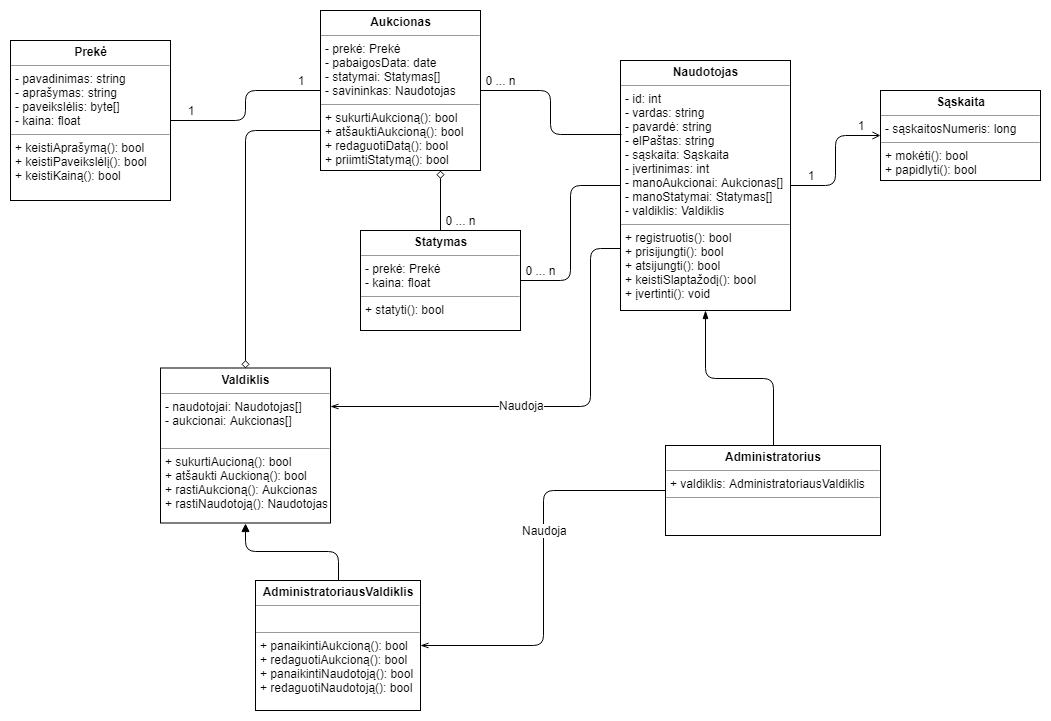
\includegraphics[width=\linewidth]{img/umlClassDiagram.png}
		\label{fig:usecase}
		\caption{Struktūrinis dalykinės srities modelis}
	\end{figure}
	\noindent
	\textbf{Esybių sąrašas:} \\
	1. Naudotojas - esybė, atsakinga už naudotojo duomenų saugojimą, jo valdymą\\
	2. Administratorius - naudotojo funkcionalumą išplečianti esybė, suteikianti galimybę atlikti administratoriaus operacijas\\
	3. Sąskaita - kiekvienam naudotojui priklausanti esybė, sauganti informaciją apie naudotojo sąskaitą bei atliekanti mokėjimo operacijas sistemoje\\
	4. Valdiklis - esybė, atsakinga už visos aukciono sistemos valdymą bei duomenų saugojimą\\
	5. Administratoriaus Valdiklis - išplėstinė valdiklio esybė, papildyta administratoriui reikalingu funkcionalumu\\
	6. Aukcionas - esybė, atsakinga už aukciono informacijos saugojimą bei jo valdymą\\
	7. Statymas - esybė, aprašanti bei sauganti informaciją apie atliktą statymą\\
	8. Prekė - esybė, apibūdinanti bei sauganti informaciją apie aukcione parduodamą prekę\\
	
	\newpage
	\newpage
	\section{UŽDUOTYS}
	Šioje dokumento dalyje yra pateikiamos sistemos atliekamos užduotys  (\ref{fig:usecase} pav.) Pateikiamas pagrindinis scenarijus ir alternatyvūs.
	\begin{figure}[H]
		\centering
		\includegraphics[width=\linewidth]{img/UseCaseDiagram.png}
		\label{fig:usecase}
		\caption{Sistemoje atliekamos užduotys}
	\end{figure}
	
	\subsection{Užduotis - Registruotis}
	Skyriuje pateikiamas užduoties registruotis aprašymas.\\
	\textbf{Užduotis:}  Registruotis \\
	\textbf{Scenarijus:} Naudotojas prisijungimo lange paspaudžia mygtuką registruotis. Sistema atidaro registracijos langą. Naudotojas suveda prisijungimo vardą, slaptažodį, pakartonai slaptažodį, el. paštą (visi laukai privalomi), spaudžia registruotis. Sistema patikrina įvestus duomenis ir pateikia pranešimą apie sėkmingą registraciją.\\
	\textbf{Alternatyvūs scenarijai:}\\
	\begin{enumerate}
		\item Jei naudotojas neįvedė bent vieno iš privalomų laukų, sistema išmeta pranešimą, jog privaloma užpildyti visus laukus.
		\item Jei naudotojo įvestas el. pašto adresas jau egzistuoja sistemoje, pastaroji išmeta pranešimą apie jau egzistuojantį el. pašto adresą.
		\item Jei naudotojo įvestas prisijungimo vardas jau egzistuoja sistemoje, pastaroji išmeta pranešimą apie jau egzistuojantį sistemos naudotoją su tokiu prisijungimo vardu. 
		\item Jei naudotojo įvestas slaptažodis ir pakartotinas slaptažodis nesutampa, sistema išmeta pranešimą apie nesutampančius įvestus slaptažodžius. 
		\item Jei naudotojas neužbaigęs registracijos paspaudžia atšaukti, sistema neišsaugo duomenų ir grąžina naudotoją į prisijungimo langą. 
	\end{enumerate}
	\textbf{Nuoroda į reikalavimą: } [FR 2]\\
	
	\subsection{Užduotis - Prisijungti}
	Skyriuje pateikiamas užduoties prisijungti aprašymas.\\
	\textbf{Užduotis:}  Prisijungti \\
	\textbf{Scenarijus:} Naudotojas prisijungimo lange savo suveda prisijungimo vardą ir slaptažodį spaudžia prisijungti. Sistema patikrina ar prisijungimo duomenys teisingi ir nukreipia į naudotojo pagrindinį langą. \\
	\textbf{Alternatyvūs scenarijai:}
	\begin{enumerate}
		\item Jei naudotojas neįvedė bent vieno iš privalomų laukų, sistema išmeta pranešimą, jog privaloma užpildyti visus laukus.
		\item Jei naudotojo įvestas prisijungimo vardas ir slaptažodis nesutampa su jokiais duomenimis sistemoje, pastaroji išmeta pranešimą apie klaidingai suvestus duomenis.
		\item Jei naudotojas neužbaigęs registracijos paspaudžia atšaukti, sistema neišsaugo duomenų ir grąžina naudotoją į prisijungimo langą. 
	\end{enumerate}
	\textbf{Nuoroda į reikalavimą: } [FR 3]
	
	\subsection{Užduotis - Atsijungti}
	Skyriuje pateikiamas užduoties atsijungti aprašymas.\\
	\textbf{Užduotis:}  Atsijungti \\
	\textbf{Scenarijus:} Prisijungęs naudotojas paspaudžia mygtuką atsijungti, sistema atjungia naudotoją, išmeta pranešimą apie sėkmingą atsijungimą, bei atidaro prisijungimo langą. \\
	\textbf{Alternatyvūs scenarijai:}
	\begin{enumerate}
		\item Jei naudotojas išjungė sistemą neatsijungęs, sistema atjungia vartotoją automatiškai. 
		\item Jei naudotojo nepavyko atjungti, sistema išmeta pranešimą, jog nepavyko atjungti naudotojo. 
	\end{enumerate}
	\textbf{Nuoroda į reikalavimą: } [FR 4]
	
	\subsection{Užduotis - Pakeisti slaptažodį}
	Skyriuje pateikiamas užduoties pakeisti slaptažodį aprašymas.\\
	\textbf{Užduotis:}  Pakeisti slaptažodį \\
	\textbf{Scenarijus:} Prisijungęs naudotojas paspaudžia mygtuką redaguoti savo duomenis, sistema atidaro naudotojo profilį, šiame lange naudotojas spaudžia keisti slaptažodį. Sistema atidaro slaptažodžio keitimo formą. Naudotojas suveda savo seną slaptažodį, naują slaptažodį, bei pastarąjį pakartoja. Sistema patikrina duomenis ir išmeta pranešimą apie sėkmingai pakeistą slaptažodį. \\
	\textbf{Alternatyvūs scenarijai:}
	\begin{enumerate}
		\item Jei naudotojo įvestas senas slaptažodis neatitinka, arba įvesti nauji slaptažodžiai nesutampa, sistema išmeta klaidos pranešimą apie klaidingai suvestus duomenis. 
		\item Jei naudotojo slaptažodžio nepavyko pakeisti, sistema išmeta pranešimą, jog slaptažodžio pakeisti nepavyko. 
	\end{enumerate}
	\textbf{Nuoroda į reikalavimą: } [FR 5]
	
	\subsection{Užduotis - Peržiūrėti aukcionus}
	Skyriuje pateikiamas užduoties peržiūrėti aukcionus aprašymas.\\
	\textbf{Užduotis:}  Peržiūrėti aukcionus \\
	\textbf{Scenarijus:} Kiekvienas sistemos naudotojas pagrindiniame puslapyje mato visus aktyvius aukcionus išrykiuotus pagal didėjantį aukciono likusį laiką. Sistemos administratorius mato ne tik aktyvius, bet ir pasibaigusius aukcionus. Prisijungęs naudotojas mato mygtuką daugiau informacijos. \\
	\textbf{Alternatyvūs scenarijai:}
	\begin{enumerate}
		\item Jei sistemoje nėra nei vieno aktyvaus aukciono, pagrindiniame puslapyje skelbiamas pranešimas, jog aktyvių aukcionių šiuo metu nėra. 
	\end{enumerate}
	\textbf{Nuoroda į reikalavimą: } [FR 7], [FR10]
	
	\subsection{Užduotis - Sukurti aukcioną}
	Skyriuje pateikiamas užduoties sukurti aukcioną aprašymas.\\
	\textbf{Užduotis:}  Sukurti aukcioną \\
	\textbf{Scenarijus:}  Prisijungęs naudotojas spaudžia mygtuką prekės įkėlimas. Sistema atidaro prekės įkėlimo/aukciono sukūrimo formą. Naudotojas suveda duomenis apie prekę: pavadinimas, aprašymas, pradinė suma, aukciono laikas, įkelia nuotraukas. Suvedęs visus duomenis naudotojas spaudžia patvirtinti. Sistema patikrina duomenis, išmeta pranešimą apie aukciono sukūrimą ir atidaro sukurtą aukcioną.\\
	\textbf{Alternatyvūs scenarijai:}
	\begin{enumerate}
		\item Jei naudotojas neužpildė kažkurio lauko sistema išmeta klaidos pranešimą su prašymu užpildyti visus laukus. 
		\item Jei naudotojas uždarė langą arba paspaudė atšaukti, jokie įvesti duomenys neišsaugojami, naudotojas grąžinamas į pagrindinį puslapį. 
		\item Jei nepavyko atnaujinti aukciono sistema išmeta klaidos pranešimą, jog nepavyko sukurti aukciono, bei grąžina naudotoją į pagrindinį puslapį. 
	\end{enumerate}
	\textbf{Nuoroda į reikalavimą: } [FR 8]
	
	\subsection{Užduotis - Pateikti statymą}
	Skyriuje pateikiamas užduoties pateikti statymą aprašymas.\\
	\textbf{Užduotis:}  Pateikti statymą \\
	\textbf{Scenarijus:}  Prisijungęs naudotojas pasirinkęs norimą aktyvų aukcioną spaudžia statyti. Sistema atidaro kainos laukelį. Naudotojas suveda norimą sumą, kuri yra ne didesnė nei jo turimi pinigai sąskaitoje ir nemažesnė, nei paskutinis statymas, ir spaudžia patvirtinti. Sistema patikrina duomenis ir išmeta pranešimą apie sėkmingai pateiktą statymą. \\
	\textbf{Alternatyvūs scenarijai:}
	\begin{enumerate}
		\item Jei naudotojo įvesta kaina yra didesnė, nei jo turimi pinigai sąskaitoje, sistema išmeta pranešimą, jog įvesta suma yra per didelė, nei jo turimi pinigai. 
		\item Jei naudotojo įvesta kaina yra mažesnė, nei kito naudotojo pasiūlyta arba mažesnė nei pradinė kaina, sistema išmeta pranešimą, jog pasiūlyta kaina yra mažesnė, nei jau esanti prekės kaina. 
		\item Jei kainos laukelis nebuvo užpildytas, sistema išmeta pranešimą, jog privaloma užpildyti visus laukus. 
		\item Jei statymo nepavyko užregistruoti, išmetamas klaidos pranešimas, jog įvyko klaida ir statymas nebuvo užfiksuotas. 
	\end{enumerate}
	\textbf{Nuoroda į reikalavimą: } [FR 9]
	
	\subsection{Užduotis - Koreguoti aukcioną}
	Skyriuje pateikiamas užduoties koreguoti aukcioną aprašymas.\\
	\textbf{Užduotis:}  Koreguoti aukcioną \\
	\textbf{Scenarijus:}  Prisijungęs naudotojas atsidaro savo profilį, kur gali matyti visus tik jo paties sukurtus aukcionus, pasirenka aukcioną, kurį nori koreguoti, spaudžia mygtuką redaguoti. Atidaromas aukciono langas. Naudotojas gali pakeisti pavadinimą, aprašymą, pradinę kainą, jei dar nėra įvykdytų statymų šiame aukcione, pridėti arba pakeisti nuotraukas. Pakeitęs norimus laukus naudotojas spaudžia patvirtinti. Sistema patikrina duomenis ir informuoja apie sėkmingai atnaujintą aukcioną, grąžina naudotoją į jo profilį.  \\
	\textbf{Alternatyvūs scenarijai:}
	\begin{enumerate}
		\item Jei naudotojas neužpildė kažkurio lauko sistema išmeta klaidos pranešimą su prašymu užpildyti visus laukus. 
		\item Jei nepavyko atnaujinti aukciono sistema išmeta klaidos pranešimą, jog nepavyko atnaujinti aukciono, bei grąžina naudotoją į jo profilio puslapį. 
		\item Jei naudotojas uždarė langą arba paspaudė atšaukti, jokie įvesti duomenys neišsaugojami, naudotojas grąžinamas į jo profilio puslapį. 
	\end{enumerate}
	\textbf{Nuoroda į reikalavimą: } [FR 9]
	
	\subsection{Užduotis - Priimti statymą}
	Skyriuje pateikiamas užduoties priimti statymą aprašymas.\\
	\textbf{Užduotis:}  Priimti statymą \\
	\textbf{Scenarijus:}  Pasibaigus aukciono laikui naudotojui atsiunčiamas pranešimas su didžiausio statymo verte, bei stačiusiojo duomenimis. Naudotojas spaudžia peržiūrėti. Sistema atidaro aukciono puslapį su visa informacija, vartotojas spaudžia patvirtinti kaip pasibaigusį.  \\
	\textbf{Alternatyvūs scenarijai:}
	\begin{enumerate}
		\item Jei pasibaigus aukcionui, prekė nebuvo nupirkta, sistema atsiunčia pranešimą su siūlymu atnaujinti aukcioną. 
		\item Jei naudotojas nepatvirtino aukciono sėkmingos pabaigos, sistema apriboją naudotojo veiksmus, kol aukcionas nebus patvirtintas kaip pabaigtas. 
	\end{enumerate}
	\textbf{Nuoroda į reikalavimą: } [FR 9]
	
	\subsection{Užduotis - Įvertinti pardavėją}
	Skyriuje pateikiamas užduoties įvertinti pardavėją statymą aprašymas.\\
	\textbf{Užduotis:}  Įvertinti pardavėją \\
	\textbf{Scenarijus:}  Sėkmingai pasibaigus aukcionui, gavus prekę, laimėjęs aukcioną naudotojas savo profilyje spaudžia patvirtinti, jog gavo prekę. Sistema išmeta pardavėjo įvertinimo formą, kurioje naudotojas užpildo pateiktus laukus apie prekės būklę, pardavėjo komunikaciją, spaudžia patvirtinti. Sistema patikrina duomenis ir pateikia pranešimą apie sėkmingai užregistruotus duomenis. \\
	\textbf{Alternatyvūs scenarijai:}
	\begin{enumerate}
		\item Jei naudotojas neužpildė kažkurio lauko sistema išmeta klaidos pranešimą su prašymu užpildyti visus laukus. 
		\item Jei naudotojas uždarė langą arba paspaudė atšaukti, jokie įvesti duomenys neišsaugojami, naudotojas grąžinamas į jo profilio puslapį. 
	\end{enumerate}
	\textbf{Nuoroda į reikalavimą: } [FR 9]
	
	\subsection{Užduotis - Peržiūrėti narius}
	Skyriuje pateikiamas užduoties peržiūrėti narius aprašymas.\\
	\textbf{Užduotis:}  Peržiūrėti narius \\
	\textbf{Scenarijus:}  Prisijungęs naudotojas, pasirinkęs bet kurį aukcioną, paspaudžia mygtuką peržiūrėti pardavėją. Sistema atidaro pardavėjo profilį. Sistemos administratorius pasirenka punktą peržiūrėti narius. Sistema atidaro visą narių sąrašą. Administratorius pasirenka dominantį narį ir spaudžia mygtuką daugiau informacijos. Sistema atidaro naudotojo profilį. \\
	\textbf{Alternatyvūs scenarijai:}
	\begin{enumerate}
		\item Jei sistemai nepavyko parodyti kito nario profilio, sistema išmeta klaidos pranešimą ir grąžina naudotoją į pagrindinį puslapį. 
	\end{enumerate}
	\textbf{Nuoroda į reikalavimą: } [FR 11]
	
	\subsection{Užduotis - Koreguoti naudotojų sąrašą}
	Skyriuje pateikiamas užduoties koreguoti naudotojų sąrašą aprašymas.\\
	\textbf{Užduotis:}  Koreguoti naudotojų sąrašą \\
	\textbf{Scenarijus:} Sistemos administratorius pasirenka punktą peržiūrėti narius. Sistema atidaro visą narių sąrašą. Administratorius pasirenka dominantį narį ir spaudžia mygtuką daugiau informacijos. Sistema atidaro naudotojo profilį. Administratorius pasirenka - pašalinti narį arba užblokuoti narį. Sistema išmeta informacijos langą, su priežastimis, administratorius pasirenka priežastį ir spaudžia patvirtinti. Sistema pateikia pranešimą apie sėkmingą naudotojo pašalinimą/užblokavimą, jei naudotojas pašalinamas - visi aktyvūs aukcionai tampa nebeaktyviais, jei naudotojas užblokuojamas, jo aukcionai yra užšaldomi tokiam laikui, kuriam yra užblokuojamas naudotojas. Visi tokio naudotojo statymai atimami, t.y. grąžinamas aukščiausias kito naudotojo statymas. \\
	\textbf{Alternatyvūs scenarijai:}
	\begin{enumerate}
		\item Jei sistemai nepavyko pašalinti naudotojo arba jo užblokuoti, sistema išmeta klaidos pranešimą ir grąžina administratorių į narių sąrašą. 
		\item Jei administratorius nepasirinko priežasties ir/arba laiko, sistema išmeta pranešimą apie privalomus užpildyti laukus. 
	\end{enumerate}
	\textbf{Nuoroda į reikalavimą: } [FR 11]
	
	\subsection{Užduotis - Koreguoti aukcionus}
	Skyriuje pateikiamas užduoties koreguoti aukcionus aprašymas.\\
	\textbf{Užduotis:}  Koreguoti aukcionus \\
	\textbf{Scenarijus:} Prisijungusiam sistemos administratoriui pateikiamas visų aukcionų sąrašas. Administratorius pasirenka dominantį aukcioną. Sistema atidaro visą informaciją apie aukcioną Spaudžia mygtuką pašalinti arba užšaldyti, sistema atidaro papildomą langą su priežastimis ir laiko pasirinkimu (jei užšaldomas). Administratorius užpildo laukus ir spaudžia patvirtinti. Sistema išmeta pranešimą apie sėkmingai užšaldytą/panaikintą aukcioną.\\
	\textbf{Alternatyvūs scenarijai:}
	\begin{enumerate}
		\item Jei sistemai nepavyko pašalinti aukciono arba jo užšaldyti, sistema išmeta klaidos pranešimą ir grąžina administratorių į aukcionų sąrašą. 
		\item Jei administratorius nepasirinko priežasties ir/arba laiko, sistema išmeta pranešimą apie privalomus užpildyti laukus. 
	\end{enumerate}
	\textbf{Nuoroda į reikalavimą: } [FR 10]
	
	\subsection{Užduotis - Peržiūrėti taisykles}
	Skyriuje pateikiamas užduoties peržiūrėti taisykles aprašymas.\\
	\textbf{Užduotis:}  Peržiūrėti taisykles \\
	\textbf{Scenarijus:}  Prisijungęs naudotojas paspaudžia taisyklės. Sistema atidaro taisyklių langą. \\
	\textbf{Alternatyvūs scenarijai:}
	\begin{enumerate}
		\item Jei sistemai nepavyko atidaryti taisyklių lango, sistema išmeta klaidos pranešimą ir grąžina naudotoją į pagrindinį puslapį. 
	\end{enumerate}
	\textbf{Nuoroda į reikalavimą: } [FR 6]
	
	\subsection{Užduotis - Papildyti sąskaitą}
	Skyriuje pateikiamas užduoties papildyti sąskaitą aprašymas.\\
	\textbf{Užduotis:}  Papildyti sąskaitą \\
	\textbf{Scenarijus:}  Prisijungęs naudotojas savo profilyje pasirenka papildyti sąskaitą. Sistema atidaro papildymo langą. Naudotojas užpildo reikiamus duomenis, spaudžia patvirtinti. Sistema praneša apie sėkmingai papildytą sąskaitą.  \\
	\textbf{Alternatyvūs scenarijai:}
	\begin{enumerate}
		\item Jei naudotojas neužpildė kažkurio privalomo lauko, sistema išmeta klaidos pranešimą su prašymu užpildyti visus laukus. 
		\item Jei sistemai nepavyko papildyti sąskaitos, sistema išmeta klaidos pranešimą ir grąžina naudotoją į jo profilį. 
	\end{enumerate}
	\textbf{Nuoroda į reikalavimą: } [FR 12]
	
	\subsection{Reikalavimų - užduočių atsekamumo matrica}
	Skyriuje pateikiama reikalavimų - užduočių atsekamumo matrica. Parodoma, kokios užduotys dalyvauja funkcinių reikalavimų įgyvendinime.\\
	\begin{figure}[H]
		\centering
		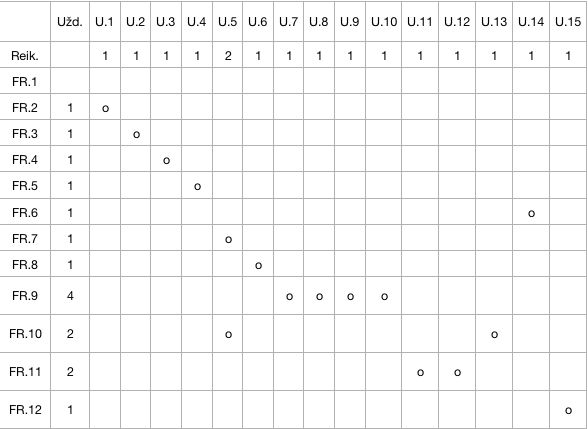
\includegraphics[width=\linewidth]{img/matrix.png}
		\label{fig:matrix}
		\caption{Reikalavimų - užduočių atsekamumo matrica}
	\end{figure}
	
	\newpage
	
	\section{Robastiškumo analizė}
	Šioje dokumentoje dalyje yra pateikiami robastiškumo analzės diagramos kiekvienai aprašytai užduočiai.
	\subsection{Registracija}
		\begin{figure}[H]
		\centering
		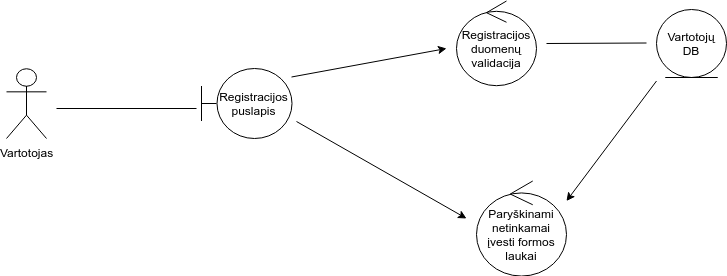
\includegraphics[width=\linewidth]{img/registracija.png}
		\label{fig:registracija}
		\caption{Registracijos puslapio robastiškumo diagrama}
	\end{figure}
	\subsection{Prisijungti}
		\begin{figure}[H]
		\centering
		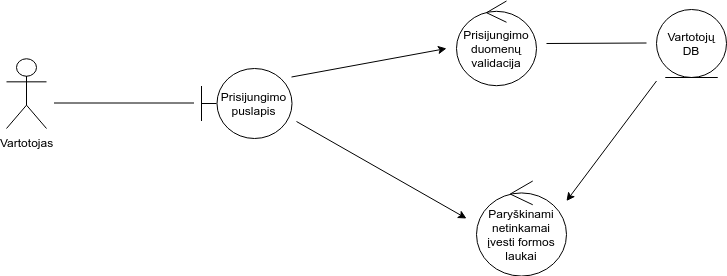
\includegraphics[width=\linewidth]{img/prisijungimas.png}
		\label{fig:prisijungimas}
		\caption{Prisijungimo puslapio robastiškumo diagrama}
	\end{figure}
	\subsection{Atsijungti}
		\begin{figure}[H]
		\centering
		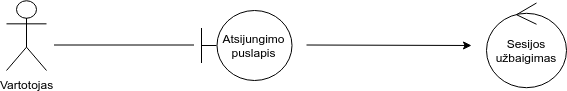
\includegraphics[width=\linewidth]{img/atsijungimas.png}
		\label{fig:atsijungti}
		\caption{Atsijungimo robastiškumo diagrama}
	\end{figure}
	\subsection{Pakeisti slaptažodį}
		\begin{figure}[H]
		\centering
		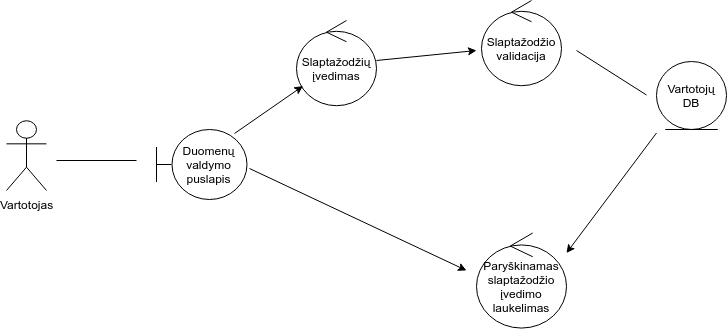
\includegraphics[width=\linewidth]{img/slaptazodis.png}
		\label{fig:slaptazodis}
		\caption{Slaptažodžio keitimo robastiškumo diagrama}
	\end{figure}
	\subsection{Peržiūrėti aukcionus}
		\begin{figure}[H]
		\centering
		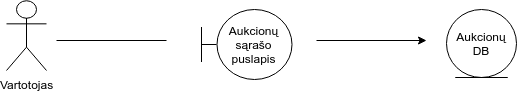
\includegraphics[width=\linewidth]{img/aukcionai.png}
		\label{fig:aukcionai}
		\caption{Aukcionų peržiūrėjimo robastiškumo diagrama}
	\end{figure}
	\subsection{Sukurti aukcioną}
		\begin{figure}[H]
		\centering
		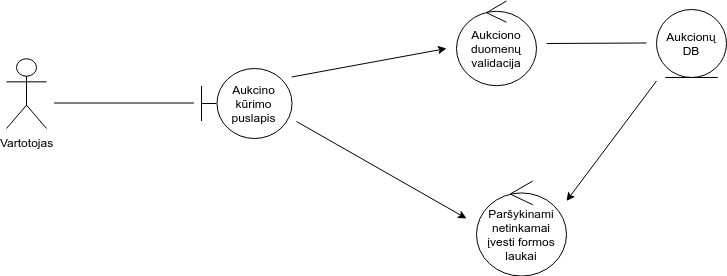
\includegraphics[width=\linewidth]{img/sukurti.png}
		\label{fig:sukurti}
		\caption{Aukciono sukūrimo robastiškumo diagrama}
	\end{figure}
	\subsection{Pateikti statymą}
		\begin{figure}[H]
		\centering
		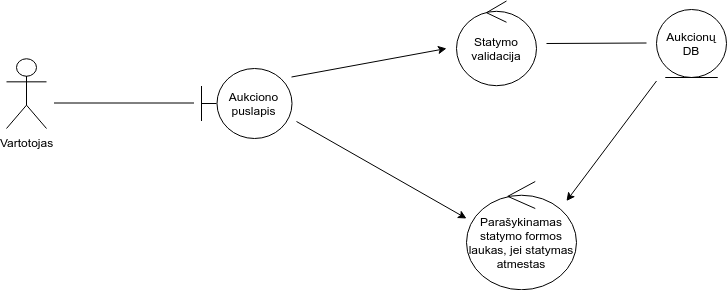
\includegraphics[width=\linewidth]{img/statymas.png}
		\label{fig:statymas}
		\caption{Statymo pateikimo robastiškumo diagrama}
	\end{figure}
	\subsection{Koreguoti aukcioną}
		\begin{figure}[H]
		\centering
		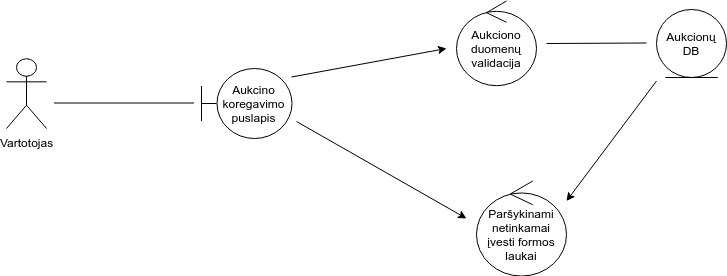
\includegraphics[width=\linewidth]{img/koreguoti.png}
		\label{fig:koregavimas}
		\caption{Aukciono koregavimo robastiškumo diagrama}
	\end{figure}
	\subsection{Priimti statymą}
		\begin{figure}[H]
		\centering
		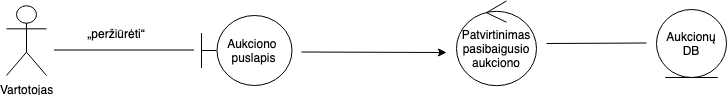
\includegraphics[width=\linewidth]{img/patvirtinti.png}
		\label{fig:takebet}
		\caption{Aukciono užbaigimo patvirtinimo robastiškumo diagrama}
	\end{figure}
	\subsection{Įvertinti pardavėją}
		\begin{figure}[H]
		\centering
		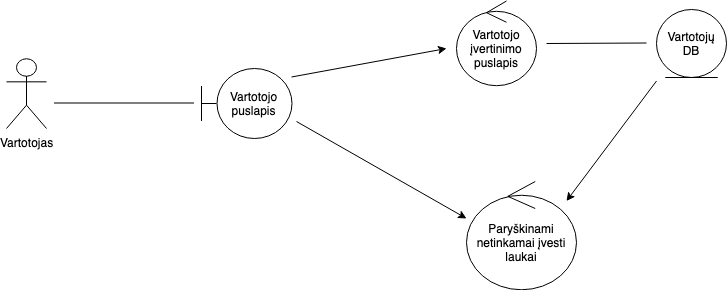
\includegraphics[width=\linewidth]{img/ivertinimas.png}
		\label{fig:ivertinimas}
		\caption{Pardavėjo įvertinimo robastiškumo diagrama}
	\end{figure}
	\subsection{Peržiūrėti narius}
		\begin{figure}[H]
		\centering
		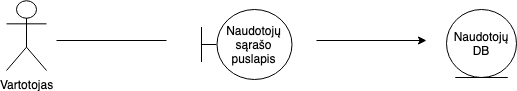
\includegraphics[width=\linewidth]{img/nariai.png}
		\label{fig:narys}
		\caption{Narių peržiūrėjimo robastiškumo diagrama}
	\end{figure}
	\subsection{Koreguoti naudotojų sąrašą}
		\begin{figure}[H]
		\centering
		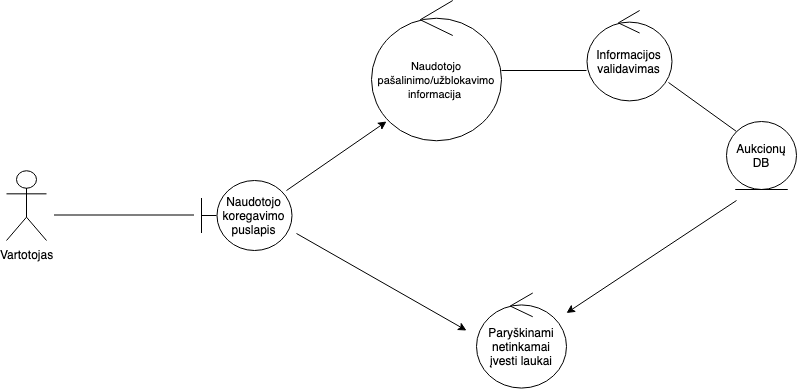
\includegraphics[width=\linewidth]{img/pasalinti.png}
		\label{fig:salinti}
		\caption{Naudotojų sąrašo koregavimo robastiškumo diagrama}
	\end{figure}
	\subsection{Koreguoti aukcionus}
		\begin{figure}[H]
		\centering
		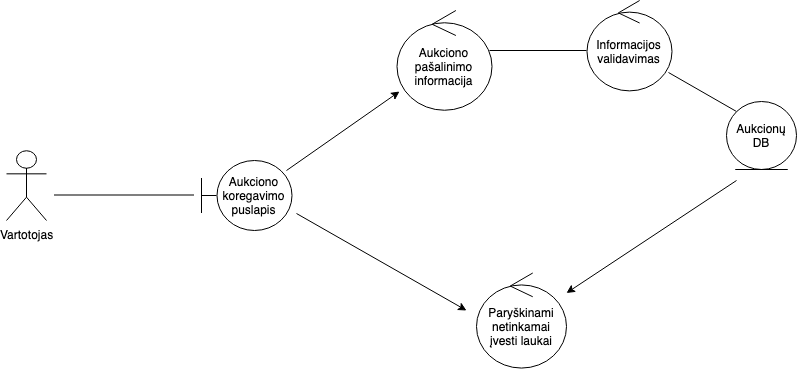
\includegraphics[width=\linewidth]{img/aukcpasalinti.png}
		\label{fig:aukckoreg}
		\caption{Aukciono koregavimo robastiškumo diagrama}
	\end{figure}
	\subsection{Peržiūrėti taisykles}
		\begin{figure}[H]
		\centering
		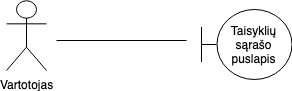
\includegraphics[width=\linewidth]{img/taisykles.png}
		\label{fig:taisykles}
		\caption{Taisyklių peržiūrėjimo robastiškumo diagrama}
	\end{figure}
	\subsection{Papildyti sąskaitą}
		\begin{figure}[H]
		\centering
		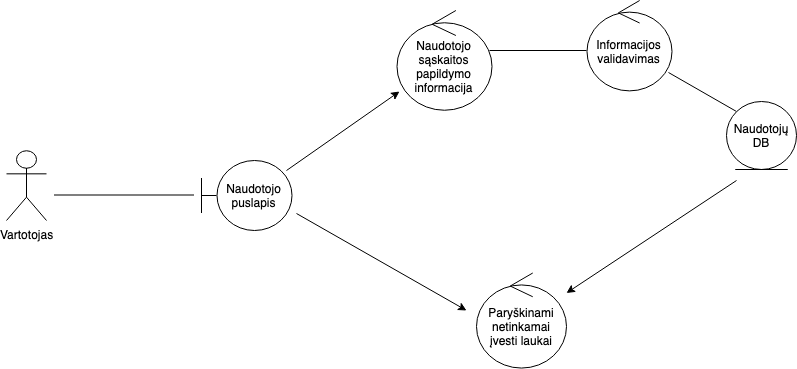
\includegraphics[width=\linewidth]{img/saskaita.png}
		\label{fig:sask}
		\caption{Sąskaitos papildymo robastiškumo diagrama}
	\end{figure}
	
	
	\newpage
	
	\sectionnonum{REZULTATAI}
	Sistema išanalizuota taikant ICONIX metodą. Pateikti funkciniai ir nefunkciniai reikalavimai, apibrėžtas struktūrinis dalykinės srities modelis. Taip pat aprašytos sistemoje atliekamos užduotys, išanalizuoti pagrindiniai ir alternatyvūs užduočių scenarijai.
	\newpage
	
	\sectionnonum{PERŽIŪROS METU RASTOS KLAIDOS}
		\begin{enumerate}
		\item Perrašyti funkciniai reikalavimai.
		\item Sustrūkturizuoti nefunkciniai reikalavimai
		\item  Pakeisti šie NFR: NFR17, NFR18, NFR23, NFR25
		\item Projektui atlikta robastiškumo analizė
	\end{enumerate}
\end{document}
